\section{Test frontend implementation of API endpoints}
We design a test frontend to demonstrate the functionality of the backend API endpoints. The frontend implements six REST API endpoints across different React components to create a complete video transcription and summarization system.
\subsection{File Upload Endpoint}
Handles uploading audio and video files from the user’s local machine. The FileUpload component provides a drag-and-drop interface with real-time progress tracking. Upon successful upload, the backend returns job and video identifiers, triggering an automatic jobs list refresh.\\
\begin{figure}[H] % Place figure here or at the top, override LaTeX's preferences
    \centering % Center the image
    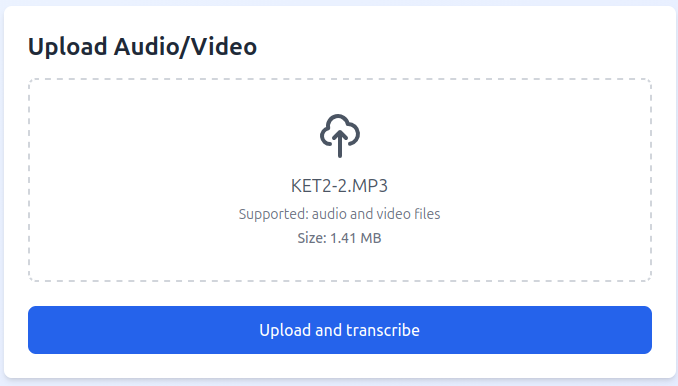
\includegraphics[scale=0.7]{experiements/image/upload.png} % Include the image, adjust width as needed
    \caption{ POST /api/upload} % Add the caption
    \label{fig:example_image} % Add a label for referencing
\end{figure}

\subsection{Jobs List Endpoint}
Retrieves paginated list of transcription jobs. Defaults to 10 jobs per page. Response includes job array and pagination metadata (total count, pages, current page). Each job shows filename, ID, status badge, timestamp, and error messages if failed.\\
\begin{figure}[H] % Place figure here or at the top, override LaTeX's preferences
    \centering % Center the image
    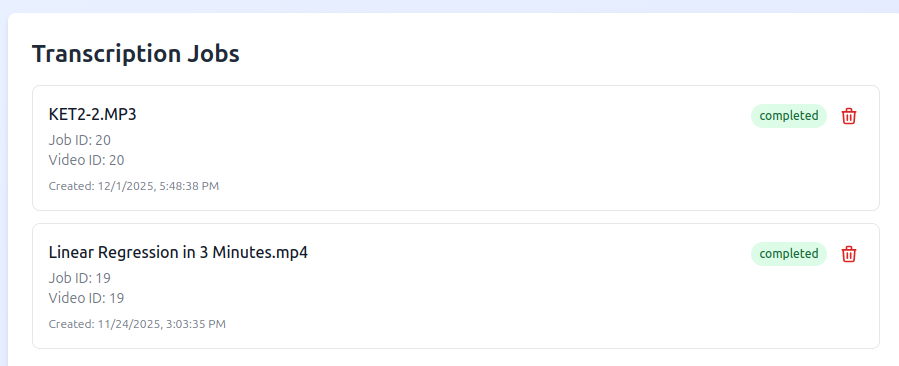
\includegraphics[scale=0.5]{experiements/image/list.png} % Include the image, adjust width as needed
    \caption{GET jobList} % Add the caption
    \label{fig:example_image} % Add a label for referencing
\end{figure}

\subsection{Delete Job Endpoint}
Permanently removes jobs from MySQL and associated transcripts from MongoDB. Displays red trash icon button with confirmation dialog to prevent accidental deletion. Auto-refreshes list on success.
\begin{figure}[H] % Place figure here or at the top, override LaTeX's preferences
    \centering % Center the image
    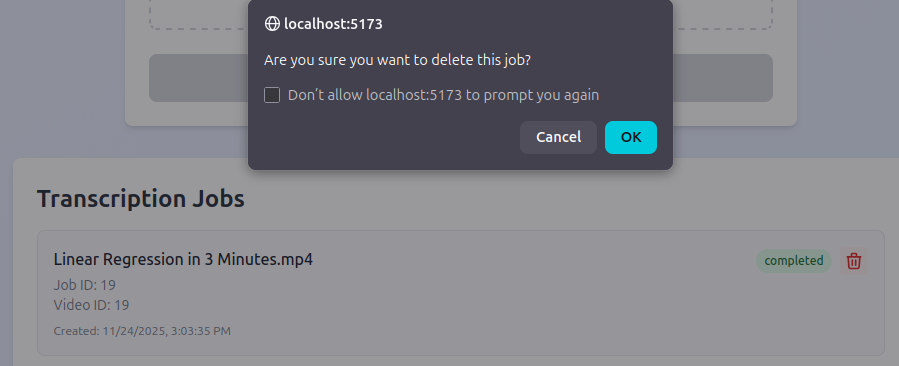
\includegraphics[scale=0.5]{experiements/image/delete.png} % Include the image, adjust width as needed
    \caption{ DELETE /api/jobs/:jobId} % Add the caption
    \label{fig:example_image} % Add a label for referencing
\end{figure}

\subsection{Get Transcript Endpoint}
Retrieves complete transcript document from MongoDB including timestamped segments, full text, language, and creation timestamp. Data is displayed in three formats: full text block, timestamped segments list, and synchronized video captions.
\begin{figure}[H] % Place figure here or at the top, override LaTeX's preferences
    \centering % Center the image
    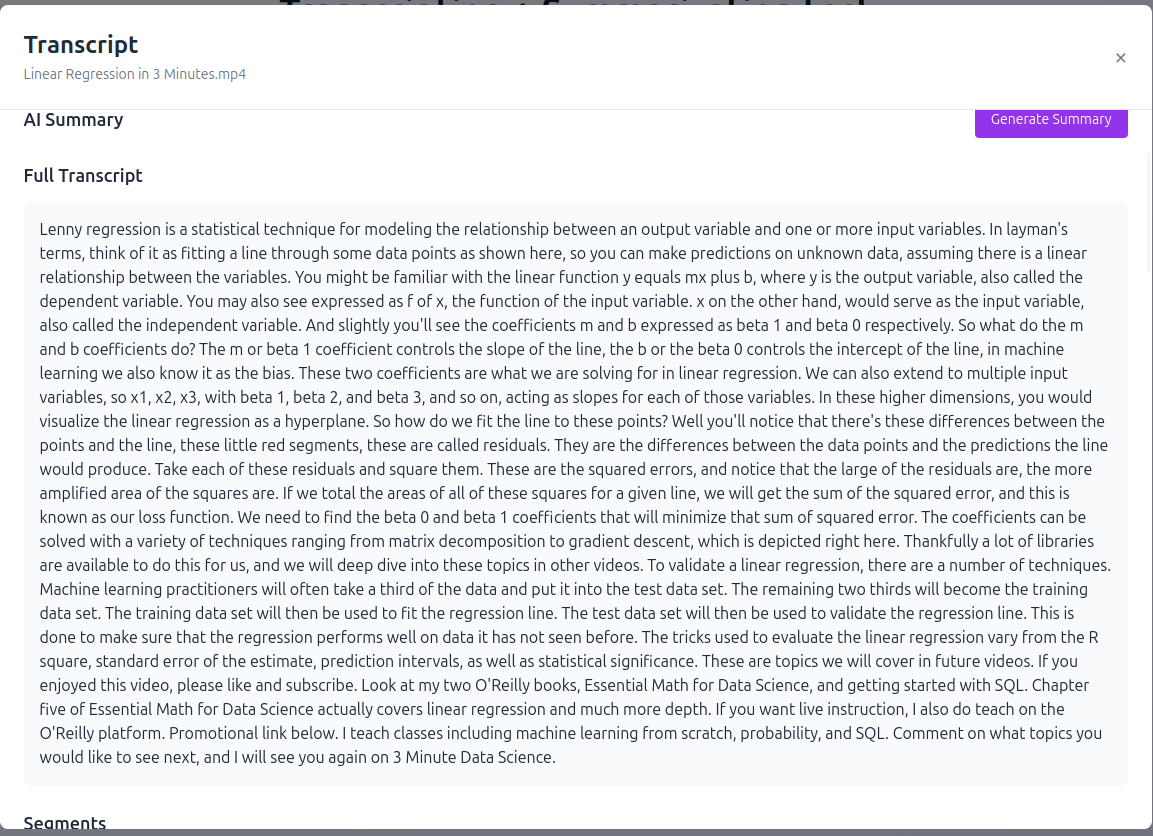
\includegraphics[scale=0.4]{experiements/image/transcript.png} % Include the image, adjust width as needed
    \caption{  GET /api/transcripts/:videoId} % Add the caption
    \label{fig:example_image} % Add a label for referencing
\end{figure}

\begin{figure}[H] % Place figure here or at the top, override LaTeX's preferences
    \centering % Center the image
    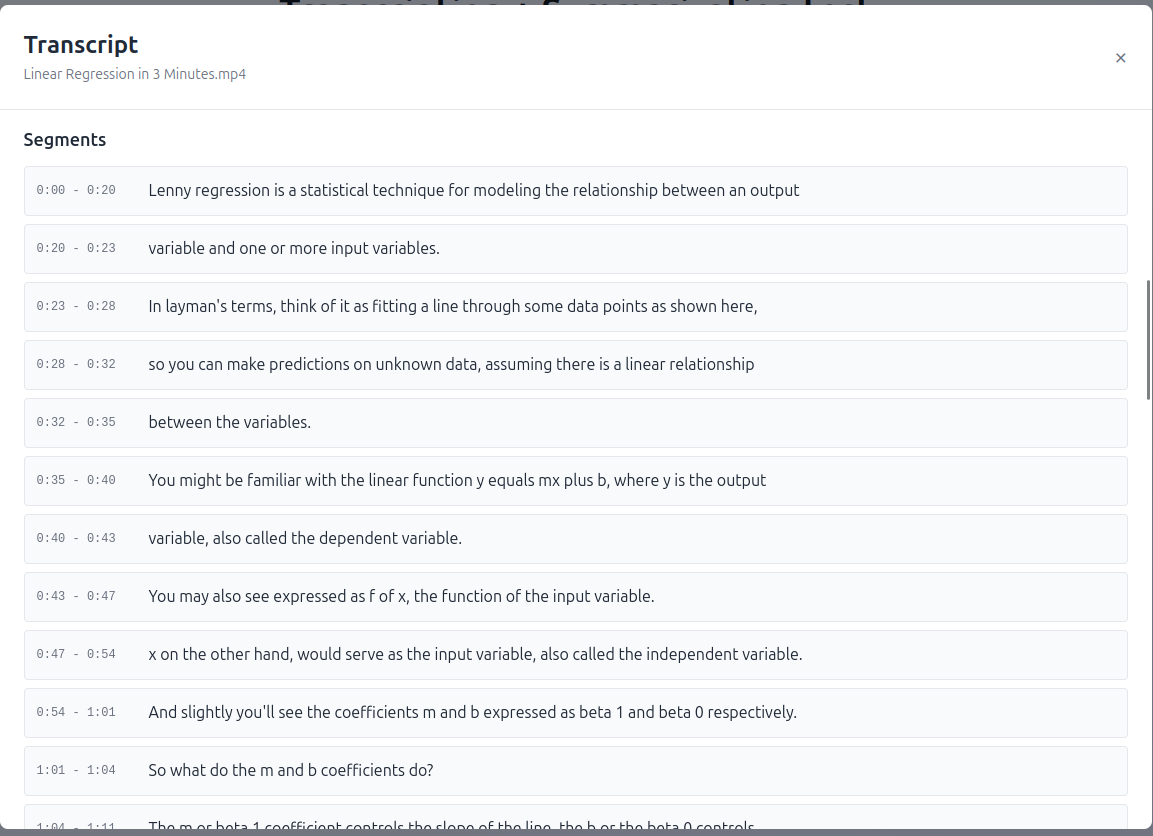
\includegraphics[scale=0.4]{experiements/image/segment.png} % Include the image, adjust width as needed
    \caption{  GET /api/transcripts/:videoId} % Add the caption
    \label{fig:example_image} % Add a label for referencing
\end{figure}

\begin{figure}[H] % Place figure here or at the top, override LaTeX's preferences
    \centering % Center the image
    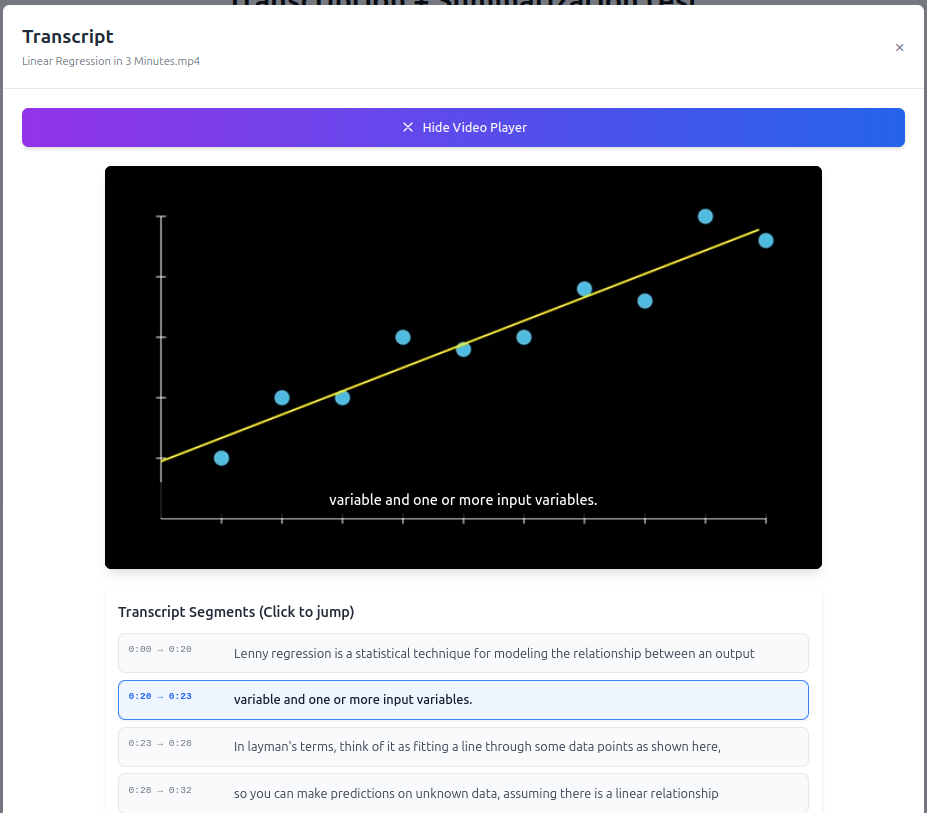
\includegraphics[scale=0.4]{experiements/image/player.png} % Include the image, adjust width as needed
    \caption{  GET /api/transcripts/:videoId} % Add the caption
    \label{fig:example_image} % Add a label for referencing
\end{figure}

\subsection{Generate Summary Endpoint}
Generates AI-powered summaries using the LED (Longformer Encoder-Decoder) model. Accepts max\_length (150) and min\_length (50) parameters. Button shows loading state during generation and changes to “Regenerate” after completion. Summary displays in purple card above transcript.
\begin{figure}[H] % Place figure here or at the top, override LaTeX's preferences
    \centering % Center the image
    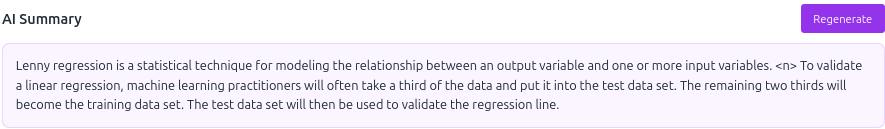
\includegraphics[scale=0.4]{experiements/image/summarize.png} % Include the image, adjust width as needed
    \caption{  POST /api/transcripts/:videoId/summarize} % Add the caption
    \label{fig:example_image} % Add a label for referencing
\end{figure}